%First Beamer Talk

\documentclass[aspectratio=169]{beamer}

% Setup appearance:

\usetheme{Darmstadt}
%\usecolortheme{lily}
%\usefonttheme[onlylarge]{structurebold}
%\setbeamerfont*{frametitle}{size=\normalsize,series=\bfseries}
%\useinnertheme{circles}


% Standard packages

\usepackage[english]{babel}
\usepackage[latin1]{inputenc}
%\usepackage{times}
\usepackage[T1]{fontenc}
\usepackage{multirow}
\usepackage{capt-of}
\usepackage{graphicx}
\usepackage{array}
\usepackage{tikz}

\setbeamertemplate{blocks}[rounded] [shadow=false]

% Some optional colors. Change or add as you see fit.
%---------------------------------------------------
 \definecolor{ualbertagreen}{HTML}{007C41}
\definecolor{ualbertagold}{HTML}{FFDB05}


% Some optional color adjustments to Beamer. Change as you see fit.
%------------------------------------------------------------------
\setbeamercolor{frametitle}{fg=ualbertagreen,bg=white}
\setbeamercolor{title}{fg=ualbertagreen,bg=white}
\setbeamercolor{author}{fg=ualbertagreen,bg=white}
\setbeamercolor{date}{fg=ualbertagreen,bg=white}
\setbeamercolor{affiliation}{fg=ualbertagreen,bg=white}
\setbeamercolor{institute}{fg=ualbertagreen,bg=white}
\setbeamercolor{local structure}{fg=ualbertagreen}
\setbeamercolor{section in toc}{fg=ualbertagreen,bg=white}
% \setbeamercolor{subsection in toc}{fg=ualbertagreen,bg=white}
\setbeamercolor{footline}{fg=ualbertagreen!50, bg=white}
\setbeamercolor{block title}{fg=ualbertagreen,bg=white}
\setbeamercolor{upper separation line head}{bg=ualbertagreen}
\setbeamercolor{lower separation line head}{bg=ualbertagold}
\setbeamercolor{middle separation line head}{bg=ualbertagold}
\setbeamercolor{frametitle}{fg=ualbertagreen,bg=white}

\setbeamercolor{section in head/foot}{bg=white,fg=ualbertagreen}
\setbeamercolor{author in head/foot}{bg=white,fg=ualbertagreen}
\setbeamercolor{date in head/foot}{bg=white,,fg=ualbertagreen}
\setbeamercolor{title in head/foot}{bg=white,fg=ualbertagreen}

\setbeamercolor{headline}{bg=white,fg=ualbertagreen}




\setbeamercolor{middle separation line head}{bg=ualbertagreen}
\setbeamercolor{alerted text}{fg=red}
\setbeamercolor{example text}{fg=black}
\setbeamercolor{structure}{fg=black}

% Various cosmetic things, though I must confess I forget what exactly these do and why I included them.
%-------------------------------------------------------------------------------------------------------
\setbeamercolor{structure}{fg=ualbertagreen}


\setbeamercolor{local structure}{parent=structure}
\setbeamercolor{item projected}{parent=item,use=item,fg=ualbertagreen,bg=white}
\setbeamercolor{enumerate item}{parent=item}

\setbeamertemplate{title page}{%
  \vbox{}
%  \vfill
    \vspace{0cm}% NEW
  \begingroup
    \centering
    \begin{beamercolorbox}[sep=8pt,center]{title}
      \usebeamerfont{title}\inserttitle\par%
      \ifx\insertsubtitle\@empty%
      \else%
        \vskip0.05em%
        {\usebeamerfont{subtitle}\usebeamercolor[fg]{subtitle}\insertsubtitle\par}%
      \fi%
    \end{beamercolorbox}%
    \vskip1em\par
    \begin{beamercolorbox}[sep=8pt,center]{author}
      \usebeamerfont{author}\insertauthor
    \end{beamercolorbox}
    \begin{beamercolorbox}[sep=8pt,center]{institute}
      \usebeamerfont{institute}\insertinstitute
    \end{beamercolorbox}
    \vspace{0.5cm}% NEW
    \begin{beamercolorbox}[sep=8pt,center]{date}
      \usebeamerfont{date}\insertdate
    \end{beamercolorbox}\vskip0.05em
%    {\usebeamercolor[fg]{titlegraphic}\inserttitlegraphic\par}
  \endgroup
%  \vfill
}


\logo{
   \tikz [remember picture,overlay]
    \node[yshift=.3cm,xshift=1.5cm] at (current page.south west)
        %or: (current page.center)
        {
\includegraphics[width=1in]{UA-ASB-COLOUR.png}};
%
\includegraphics[height=0.8cm]{UA-ASB-COLOUR.png}\vspace{220pt}
}




\setbeamertemplate{headline}{%
\leavevmode%
  \hbox{%
    \begin{beamercolorbox}[wd=\paperwidth,ht=5ex,dp=1.825ex]{white}%
    \usebeamerfont{headline}\hskip6pt\inserttitle\par%
    \insertsectionnavigationhorizontal{\paperwidth}{}{\hskip0pt plus1filll}
    \end{beamercolorbox}%
  }
}

\setbeamertemplate{sidebar right}{}


\logo{
   \tikz [remember picture,overlay]
    \node[yshift=.3cm,xshift=1.5cm] at (current page.south west)
        %or: (current page.center)
        {
\includegraphics[width=1in]{UA-ASB-COLOUR.png}};
%
\includegraphics[height=0.8cm]{UA-ASB-COLOUR.png}\vspace{220pt}
}




%\setbeamertemplate{footline}{%
%\hfill\usebeamertemplate***{navigation symbols}
%\hspace{1cm}\insertframenumber{}/\inserttotalframenumber}
\defbeamertemplate*{footline}{my footline}{%
    \ifnum\insertpagenumber=1
        \Tiny{%
            \hfill%
		\vspace*{1pt}%
            %\insertframenumber/\inserttotalframenumber \hspace*{0.1cm}%
            \newline%
            \color{ualbertagold}{\rule{\paperwidth}{0.4mm}}\newline%
            \color{ualbertagold}{\rule{\paperwidth}{.4mm}}%
        }
%    \hbox{%
%        \begin{beamercolorbox}[wd=\paperwidth,ht=.8ex,dp=1ex,center]{}%
%      % empty environment to raise height
%        \end{beamercolorbox}%
%    %}%
    %\vskip0pt%
    %no page number on the first page
    %    \Tiny{%
    %        \hfill%
   % 		\vspace*{1pt}%
    %        \color{ualbertagold}{\rule{\paperwidth}{0.4mm}}\newline%
    %        \color{ualbertagold}{\rule{\paperwidth}{.4mm}}%
%        }%
  \else%
        \Tiny{%
            \hfill%
		\vspace*{1pt}%
            \insertframenumber/\inserttotalframenumber \hspace*{0.1cm}%
            \newline%
            \color{ualbertagold}{\rule{\paperwidth}{0.4mm}}\newline%
            \color{ualbertagold}{\rule{\paperwidth}{.4mm}}%
        }%
    \fi%
}









\renewcommand{\(}{\begin{columns}}
\renewcommand{\)}{\end{columns}}
\newcommand{\<}[1]{\begin{column}{#1}}
\renewcommand{\>}{\end{column}}
%%%%%%%%%%%%%%%%%%%%%%%%%%%%%%%%%%%%%%%%%%%%%%%%%%





% Author, Title, etc.

\title[Electricity Slide Pack]
{%
  Electricity Markets%
}

\author[Leach]
{
  Andrew~Leach
}

\institute[2017]
{
  University of Alberta
 }

\date[5/28/2017]
{\today}


\newcommand{\degC}{$^o$C$\,$}
\newcommand{\co}{$\text{CO}_{2}\,$}
\newcommand{\tx}{$G_{2\times\text{CO}_2}$}
\newcommand{\Real}{\mathbb R}





% Bayliss Fancy fit image command with optional caption
\usepackage{adjustbox} % Shrink stuff

\makeatletter

\newcommand{\fitimage}[2][\@nil]{
  \begin{figure}
    \begin{adjustbox}{width=0.95\textwidth, totalheight=\textheight-2\baselineskip-2\baselineskip,keepaspectratio}
      \includegraphics{#2}
    \end{adjustbox}
    \def\tmp{#1}%
   \ifx\tmp\@nnil
      \else
      \newline{\tiny{#1}}
    \fi
  \end{figure}
}

\makeatother





% The main document


\begin{document}

\begin{frame}
   %\tikz [remember picture,overlay]
   % \node[yshift=-0.95cm,xshift=0cm] at (current page.north)
        %or: (current page.center)
        %\node[yshift=-0.75cm,xshift=4.5cm] at (current page.north west)
        %{
\includegraphics[width=3in]{UA-ASB-COLOUR.png}};
        %{
\includegraphics[width=\paperwidth]{EE_logo.png}}; \vspace{1cm}
   \titlepage
   \vfill
\end{frame}



\section{Introduction}




\begin{frame}{Why aspiring lawyers should care about electricity and what you need to know}
\begin{itemize}
\setlength\itemsep{.5em}
\item Regulatory complexity:
\begin{itemize}
\setlength\itemsep{.5em}
    \item Complex regulation, even in \textit{deregulated} jurisdictions
    \item Each part of the market has its own set of regulatory constructs (distribution, transmission, generation, retail)
\end{itemize}
\item New technology means evolving market structures:
\begin{itemize}
\setlength\itemsep{.5em}
\item Electricity is, arguably, changing faster than any other energy market
\item Alberta's electricity market in the midst of a period of market- and regulatory-driven transition
\end{itemize}
\item Economics 101 in action
\begin{itemize}
\setlength\itemsep{.5em}
\item Supply and demand curves determine prices every hour in Alberta's power market
\end{itemize}
\item The next constitutional battleground?
\begin{itemize}
\setlength\itemsep{.5em}
\item Fed/prov issues, environmental policy, section 125 jurisprudence, the oddity that is section 92(10) including the declaratory power, and POGG all come into play!
\end{itemize}
\end{itemize}
\vfill
\end{frame}


\begin{frame}

\begin{tabular}{p{\linewidth}}
    \centering
    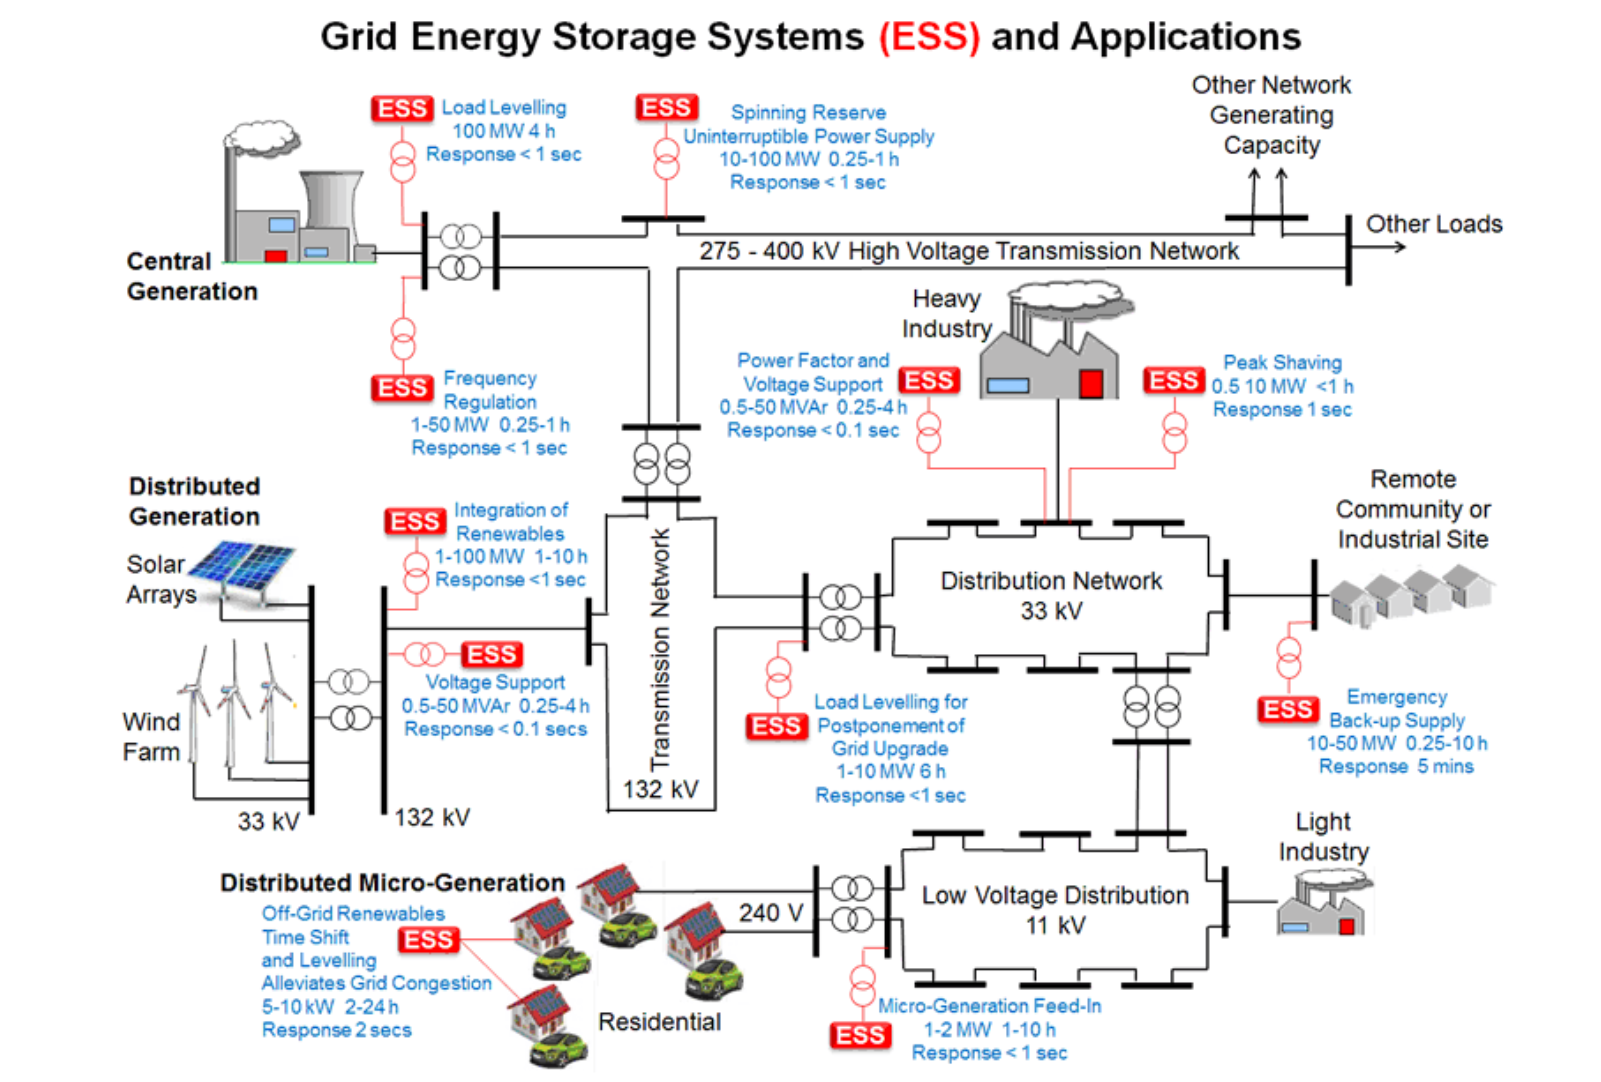
\includegraphics[width=.75\linewidth]{../images/grid_storage.png} \\[\abovecaptionskip]
  Source: \url{http://www.mpoweruk.com/grid_storage.htm}
\end{tabular}

\end{frame}

\begin{frame}{Market Participants}
\begin{itemize}
\setlength\itemsep{1.2em}
\item Generation

\item Transmission

\item Distribution

\item Ancillary Services

\item Load

\item Storage

\item Microgeneration
\end{itemize}

\vfill \end{frame}



\begin{frame}{Market Regulation in Alberta}
\begin{itemize}
\setlength\itemsep{1.7em}
\item Generation is a competitive market

\item Transmission is regulated on a cost-of-service basis

\item Distribution (local wires) is regulated on a cost-of-service basis, but retail (billing) is competitive.

\item Ancillary Services is competitive

\item Load (i.e. customers) may contract for electricity supply

\item Storage (Still a lot TBD)

\item Microgeneration (free market for self-supply)
\end{itemize}

\vfill \end{frame}


\section{Units}

\begin{frame}{Energy units - electricity}
\begin{itemize}
\setlength\itemsep{.75em}
\item Watts: measure of capacity (instantaneous production, installed capacity, or instantaneous demand)
\begin{itemize}
\setlength\itemsep{.5em}
\item Alberta system demand: 7,200-10,700 MW (megawatts or million watts)
\item Capital Power's Genessee 3 power plant has a nameplate capacity of 450 MW
\end{itemize}
\item Watt hours: measure of energy (production or demand during a given period of time; i.e. flow through)
\begin{itemize}
\setlength\itemsep{.5em}
\item Production over a day, week, month, year
\item A 7.5W LED bulb on all day (24hr) uses 180Wh of electricity (.18kWh)
\end{itemize}
\item Volts: measure of the electrical potential or the ability to convert charge to power (Watts=amps x volts)
\begin{itemize}
\setlength\itemsep{.5em}
\item Transmission lines: 150-765 kV
\item Distribution lines: 13,800 Volts
\item Household wiring: 120-240 Volts
\end{itemize}
\end{itemize}
\vfill \end{frame}

\begin{frame}{Energy Prices}
\begin{itemize}
\setlength\itemsep{.25em}
\item Electricity prices: expressed in power delivered over time
\begin{itemize}
\setlength\itemsep{.15em}
\item Cents/kilowatt-hour (c/kWh)
\item Dollars per megawatt-hour (\$/MWh)
\item Levelized costs of electricity (supply costs) in \$/MWh
\end{itemize}

\item Capacity costs are expressed in a cost per megawatt or cost of capacity
\begin{itemize}
\setlength\itemsep{.15em}
\item Genessee 3 cost approximately \$1.5 million/MW or \$1.50 per watt to build
\item Solar panel prices have declined to now lie under \$1/W of capacity
\item Balance of system costs imply that a solar system costs \$2-3/W of installed capacity
\end{itemize}
\item Other prices matter for electricity markets as well
\begin{itemize}
\setlength\itemsep{.15em}
\item Renewable energy credits (usually prices in \$/MWh)
\item Emissions credits or permits (\$/tonne)
\item Capacity payments (\$/MW)
\item GHG or other emissions permits or credits (\$/tonne)
\end{itemize}
\end{itemize}

\vfill \end{frame}


\section{Power Markets}

\begin{frame}{Regulatory characteristics}
\begin{itemize}
\setlength\itemsep{1.25em}
\item Rate-regulated or or state-owned utilities
\begin{itemize}
\setlength\itemsep{.15em}
\item EPCOR (legacy) or BC Hydro
\item PG \& E in California
\end{itemize}

\item Competitive markets
\begin{itemize}
\setlength\itemsep{.15em}
\item Energy only markets: ERCOT and Alberta
\item Energy and capacity markets: MISO, PJM
\item Real-time vs day-ahead prices: PJM and others have day-ahead market and then a real-time differences market
\item Many other design characteristic differences between restructured or competitive markets
\end{itemize}
\end{itemize}
\vfill
\end{frame}


\begin{frame}{Alberta Wholesale Energy Market Design}
\begin{itemize}
\setlength\itemsep{.25em}
\item Energy-only market
\item Real time, spot pricing, no day-ahead market
\item Single node
\item Capacity market was contemplated, but not pursued
\item Transmission
\begin{itemize}
\setlength\itemsep{.25em}
\item Regulated monopoly
\item Congestion free (no nodal pricing)
\item No transmission rights
\item Paid for (mostly) by load (consumers)
\end{itemize}
\item Ancillary services: separate, competitive market for operating reserves, transmission-must-run, load-shed and black start
\end{itemize}

\vfill
\end{frame}


\begin{frame}{Nodal Pricing Example}

\begin{tabular}{p{\linewidth}}
    \centering
    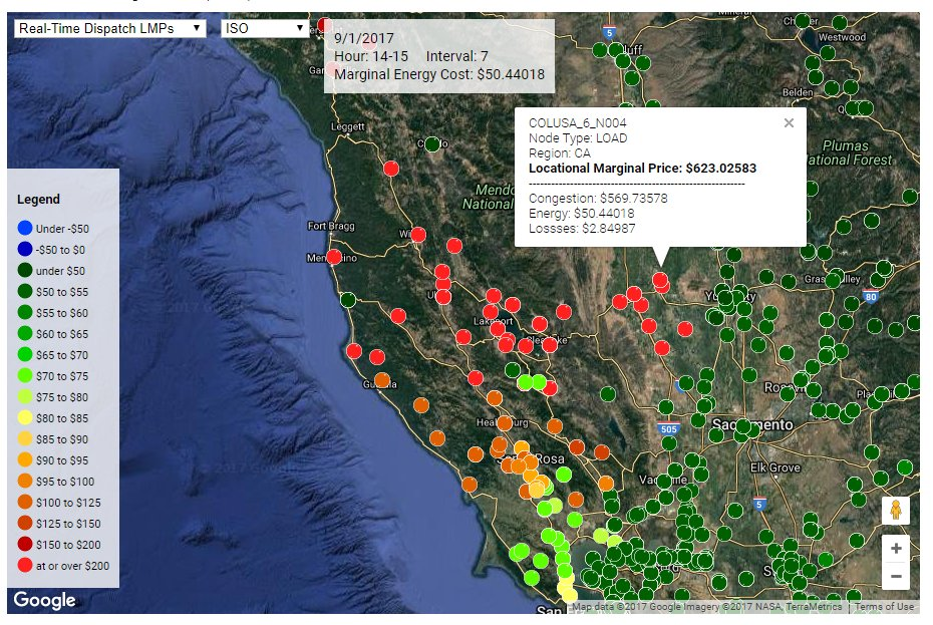
\includegraphics[width=.7\linewidth]{../images/cali_nodes.png} \\[.1\abovecaptionskip]
  Source: CAISO
\end{tabular}
\vfill
\end{frame}

\section{Wholesale Market}

\begin{frame}{The Alberta Wholesale Market}
\begin{itemize}
\item Suppliers place offers of power at particular price[-5em]
\item Demand-side bids placed for power with a maximum price
\item Supply offers are sorted from low to high
\item Demand offers are sorted from high to low
\item Marginal price is set at the price which equates supply and demand - economics 101 at work!
\item Import and renewable supply is bid-in at \$0, but everyone receives the market price
\item Export demand is bid-in at \$999, so they do not set the price directly but pay the marginal price
\item Consumer default bid allows AESO to go up merit order to meet observed demand
\end{itemize}

\vfill \end{frame}

\begin{frame}{The Merit Order}
   \fitimage{../images/merit_type.png}
   \vfill
   \end{frame}

\begin{frame}{The Merit Order}
   \fitimage{../images/merit_offer.png}
   \vfill
\end{frame}

\begin{frame}{Offers}
   \fitimage{../images/bids.png}
   \vfill
\end{frame}


\begin{frame}{Hourly Loads}
   \fitimage{../images/hourly_loads.png}
   \vfill
\end{frame}


\begin{frame}{Peak and Average Loads}
   \fitimage{../images/loads_clean.png}
   \vfill
\end{frame}


\begin{frame}{Hourly Prices}
   \fitimage{../images/hourly_prices.png}
   \vfill
\end{frame}


\begin{frame}{Prices over time}
  \fitimage{../images/peak_prices.png}
   \vfill
\end{frame}


\begin{frame}{Forward Markets}
   \fitimage{../images/forwards.png}
   \vfill
\end{frame}


\section{PPAs and the Balancing Pool}

\begin{frame}{The Balancing Pool: What on earth does/did it do?}
\fitimage[Source: Capital Power]{../images/balancingpool.png}
\vfill \end{frame}


\section{Alberta Market Evolution}

\begin{frame}{Alberta's Evolving Electricity Market}
\begin{itemize}
\setlength\itemsep{2em}
\item Capacity Market False Start
\item Coal Phase Out
\item Renewables (the REP Program and now commercial PPAs)
\item Carbon Pricing (TIER and the federal GGPPA)
\end{itemize}

\vfill \end{frame}


\begin{frame}{Costs of New Capacity Additions}
   \fitimage{../images/lcoe_22.png}
   %\\[\abovecaptionskip]  \vspace{5.5cm}
   %\tiny{See for more information: \url{https://www.lazard.com/media/451086/lazards-levelized-cost-of-energy-version-130-vf.pdf}}
   \vfill
\end{frame}


\begin{frame}{Costs of New Capacity Additions}
   \fitimage{../images/lcoe_lazard_22.png}
   \vfill
\end{frame}

\begin{frame}{New Technology}
   \fitimage{../images/ab_solar.png}
   \vfill
\end{frame}


\begin{frame}{New Technology}
   \fitimage{../images/solar.png}
   \vfill
\end{frame}

\begin{frame}{New Technology}
   \fitimage{../images/solar_year.png}
   \vfill
\end{frame}

\begin{frame}{New Technology}
   \fitimage{../images/small_solar.png}
   \vfill
\end{frame}

\begin{frame}{Price Capture by Technology}
\fitimage{../images/price_capture_renew.png}
   \vfill
\end{frame}

\begin{frame}{Evolution of Technology}
   \fitimage{../images/eia_solar.png}
   \vfill
\end{frame}



\begin{frame}{Evolution of Technology}
   \fitimage{../images/eia_coal.png}
   \vfill
\end{frame}


\begin{frame}{Evolution of Technology}
   \fitimage[Source: Lazard]{../images/lazard_decline.png}
   \vfill
\end{frame}


\begin{frame}{GHG Policy and Electricity Supply}
   \fitimage{../images/monthly_ghgs.png}
   \vfill
\end{frame}


\begin{frame}{Deeper cuts: the roles of storage and transmission}
\begin{itemize}
\setlength\itemsep{2em}
\item Renewables now offer some of the cheapest electricity we have ever seen
\item Renewables are not (generally) dispatchable
\item Renewables seasonal and/or daily generation patterns don't always match load
\item The sun is always shining / the wind is always blowing somewhere
\end{itemize}

\vfill \end{frame}



\begin{frame}{Deeper cuts: the roles of storage and transmission}
\begin{itemize}
\setlength\itemsep{2em}
\item How do we overcome the need for more transmission or storage?
\item Who will pay for the assets? How will the assets be paid for the services they provide?
\item Renewables, storage, and even transmission can erode their own value proposition - with a lot of storage or transmission in place, it's harder to see the value for storage
\item The value of transmission and storage assets may not be captured by the jurisdiction or the regulatory sector in which they are built

\end{itemize}

\vfill \end{frame}



\begin{frame}{Readings and guest speaker}
\begin{itemize}
\setlength\itemsep{2em}
\item Rivers and Dolter paper on decarbonizing Canada's supply
\item van de Biezenbos paper on transmission

\item Clean Electricity Standard discussion paper

\end{itemize}

\vfill \end{frame}




\end{document}




\begin{frame}{Price Volatility}
   \tikz [remember picture,overlay]
    \node[yshift=-.5cm,xshift=0cm] at (current page.center)
        {\includegraphics[width=.9\paperwidth]{../images/peak_prices_2000_2021.png}}; \vspace{1cm}
   \vfill
\end{frame}

\begin{frame}{Price Volatility}
   \tikz [remember picture,overlay]
    \node[yshift=-.5cm,xshift=0cm] at (current page.center)
        {\includegraphics[width=.9\paperwidth]{../images/hourly_prices_col.png}}; \vspace{1cm}
   \vfill
\end{frame}


\begin{frame}{Growth}
   \tikz [remember picture,overlay]
    \node[yshift=-.5cm,xshift=0cm] at (current page.center)
        {\includegraphics[width=.9\paperwidth]{../images/load_time.png}}; \vspace{1cm}
   \vfill
\end{frame}



\begin{frame}{Economics 101}
   \tikz [remember picture,overlay]
    \node[yshift=-.5cm,xshift=0cm] at (current page.center)
        {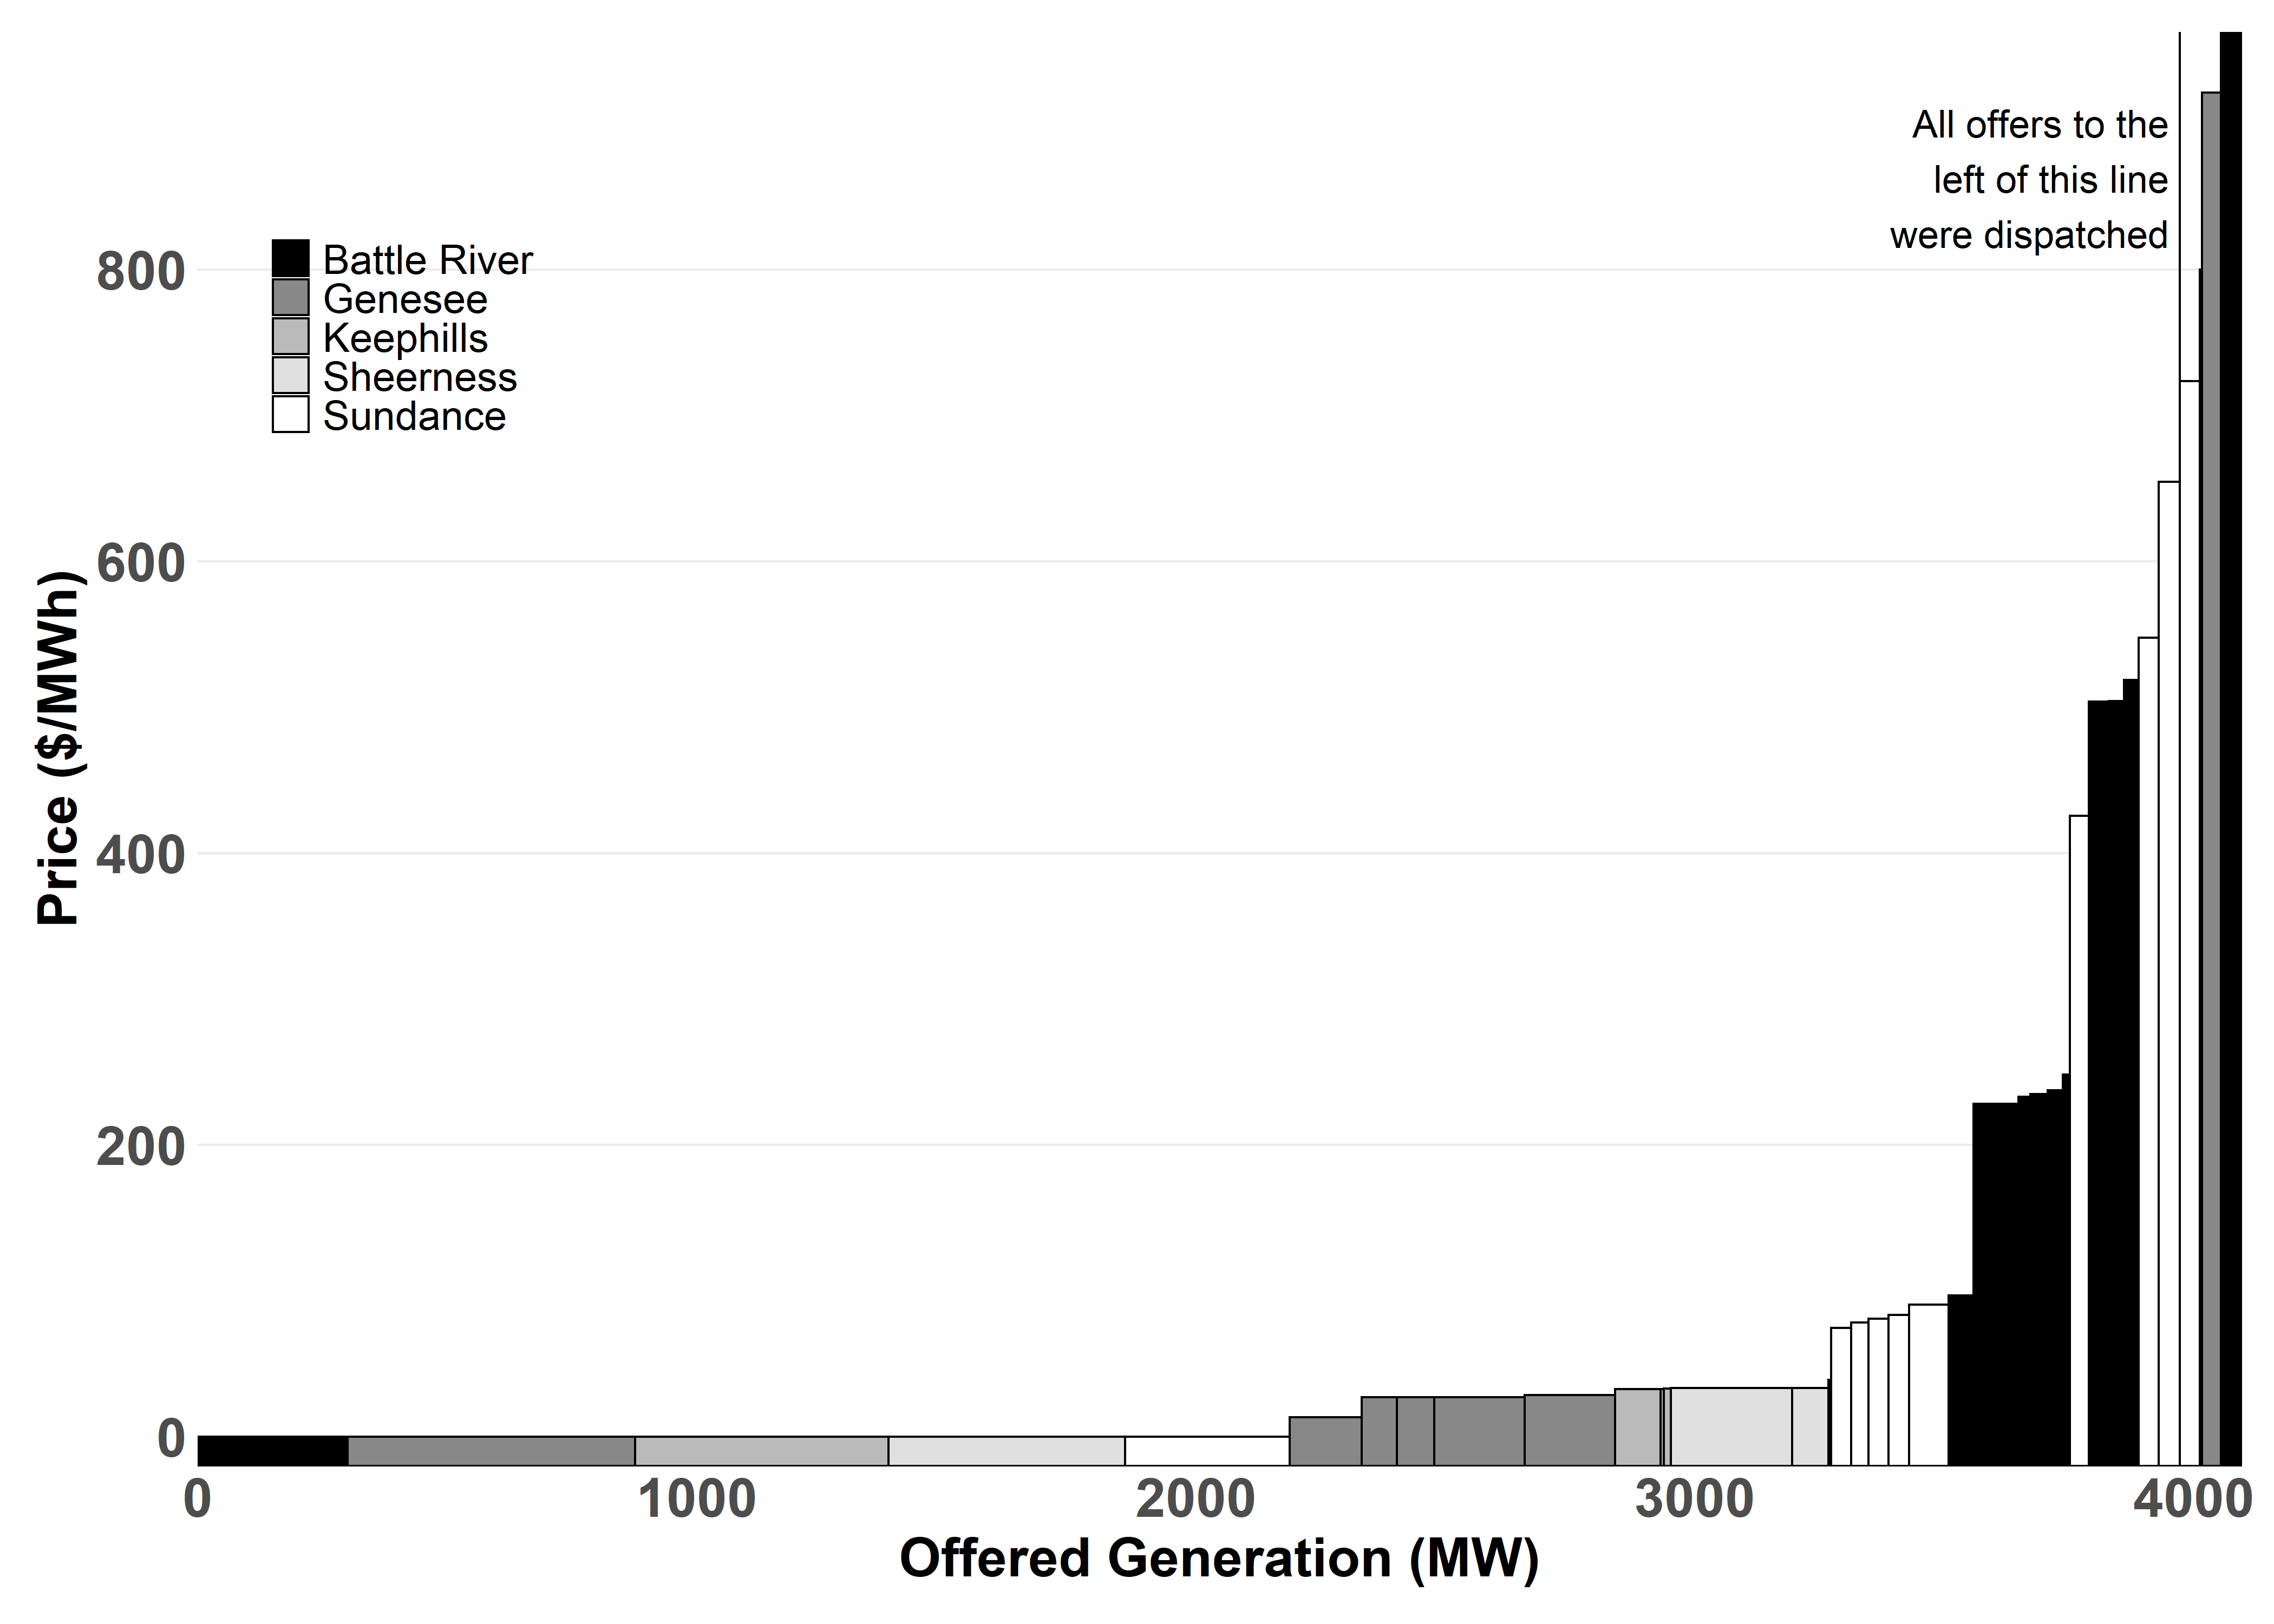
\includegraphics[width=.9\paperwidth]{../images/coal_merit.png}}; \vspace{1cm}
   \vfill
\end{frame}

\begin{frame}{Economics 101}
   \tikz [remember picture,overlay]
    \node[yshift=-.5cm,xshift=0cm] at (current page.center)
        {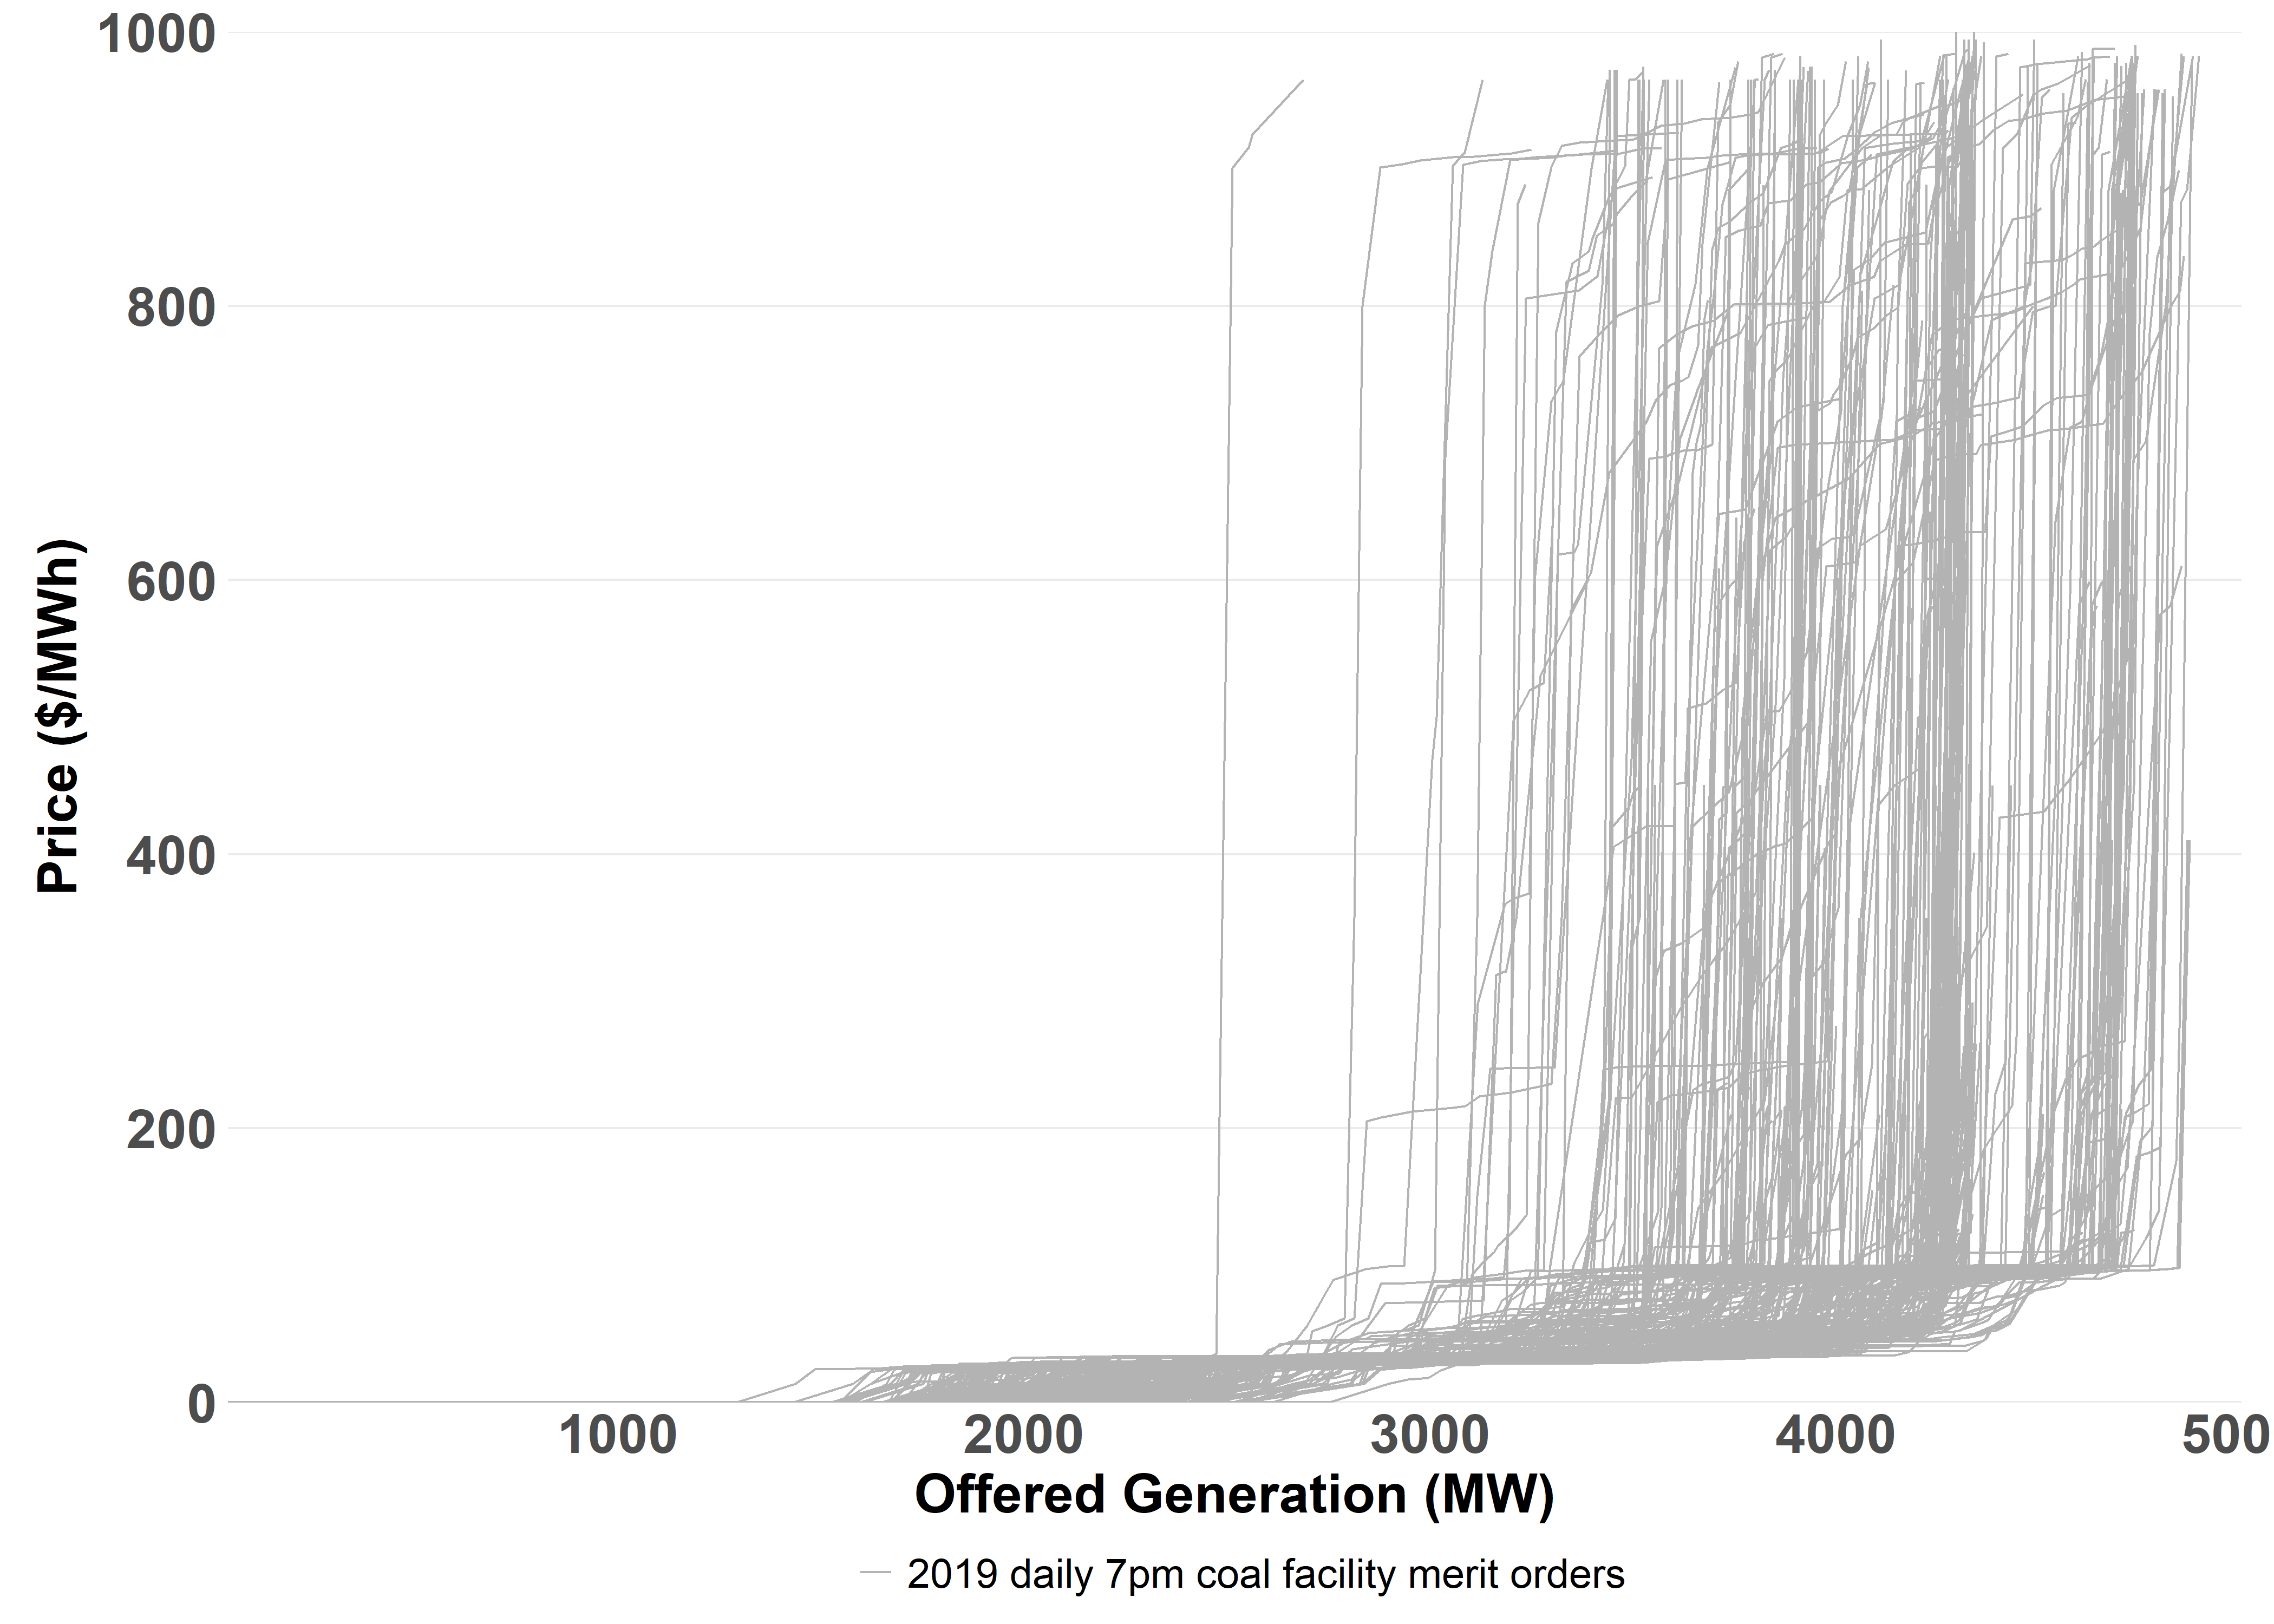
\includegraphics[width=.9\paperwidth]{../images/all_coal_merit.png}}; \vspace{1cm}
   \vfill
\end{frame}


